\chapter{Introduction}

Recent years have witnessed the rapid development of the Internet of Things (IoT) which provides ubiquitous sensing and computing capabilities to connect a broad range of things to the Internet \cite{lin2017survey}. To obtain insights on the data generated from ubiquitous IoT devices, Artificial Intelligence (AI) techniques such as Deep Learning (DL) have been widely exploited to train data models for enabling intelligent IoT applications such as smart healthcare, smart transportation and smart city \cite{mohammadi2018enabling}. \\

Traditionally, AI functions are placed in a cloud server or a data center for data learning and modeling \cite{sun2019application}, which incurs critical limitations given the huge amount of data from IoT sources. According to Cisco, there are nearly 850 ZB of data generated by all people, machines and things at the network edge by 2021. In sharp contrast, the global data center traffic is presumed reaching 20.6 ZB in 2021 \cite{cisco}. With such a tremendous growth of
IoT data at the network edge, in line with the growth in the number of devices (Fig. \ref{fig:growth}), centralizing the computation on the remote servers may be infeasible due to the required network resources and the incurred latency.

\begin{center}
\begin{minipage}[c]{\textwidth}
    \centering
    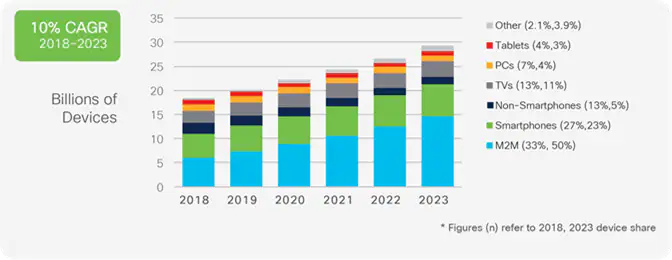
\includegraphics[width=0.8\textwidth]{contents/Chapter1/growth.png}
    \captionof{figure}{Global device and connection growth \cite{cisco2}}
    \label{fig:growth}
\end{minipage}
\end{center}

Furthermore, the use of third-party servers for AI training also raises privacy concerns, as training data may contain sensitive information such as user addresses or personal preferences \cite{granjal2015security}. It is thus highly necessary for developing innovative AI approaches to realize efficient and privacy-enhanced intelligent IoT networks and applications. \\

%\section{EU H2020 TEACHING Project}

Concurrently, both industry and society are experiencing the transformational impact of the autonomous systems revolution, empowered by automation capabilities offered by Artificial Intelligence (AI). Cyber-physical Systems of Systems (CPSoS) define a multi-faceted and dynamic environment where autonomy is fundamental to govern the complexity of interactions between the virtual and physical worlds with minimal human intervention. However, even when the most advanced degree of autonomy is exercised, the human is a variable which cannot be left out of the CPSoS equation, particularly in safety critical scenarios like autonomous transportation \cite{teachingUnipi}. \\

In this context, the TEACHING project\footnote{\url{https://teaching-h2020.eu/}} (i.e., a computing Toolkit for building Efficient Autonomous appliCations leveraging Humanistic INtelliGence) is an EU-funded project that puts forward a vision of humans at the center of autonomous CPSoS. Embracing the concept of Humanistic Intelligence, it pursues a vision where the CPSoS adapts itself by means of human feedback, achieving a mutual empowerment towards a shared goal. \\

The objective of the Project is the design, development and deployment of autonomous, adaptive and dependable CPSoS applications, allowing them to exploit a sustainable human feedback to drive, optimize and personalize the provisioning of their services. \\

This Work was done under the Human State Monitoring task of the TEACHING project, and aims to develop an efficient learning model for predicting the stress conditions of a human driver from physiological data. Being such data inherently distributed and privacy-constrained, the further challenge that we addressed was to perform the learning in a federated environment. \\

Specifically, this Work tries to improve the State of the Art (SOTA) performances of an Echo State Network (ESN) used for the prediction of the stress value of a human driving car, which acts as a proxy for adapting the driving profile. The final model is analyzed in a FL scenario to compare different FL algorithms and comparing them with SOTA performances. \\

In Chapter \ref{chapter:background} are analyzed the theoretical aspects concerning the ESN model, FL algorithms and FL applied to ESNs. In Chapter \ref{chapter:fedcurv} is explained the specific implementation of the FL algorithm FedCurv used on ESNs. In Chapter \ref{chapter:disc} is discussed the novel approach of discriminating among anomalous/not anomalous client in the federated setting. Chapter \ref{chapter:dataset} is focused on the preprocessing of the WESAD Dataset\footnote{\url{https://archive.ics.uci.edu/ml/datasets/WESAD+\%28Wearable+Stress+and+Affect+Detection\%29}} used for the experiments that are explained in Chapter \ref{chapter:experiments}. The conclusions and future works are discussed in Chapter \ref{chapter:conclusions}.